% Vector overview. Compile in paper/: xelatex fig_method_overview.tex
% Sized at the manuscript's 5.5-inch text width; body labels are 8 pt.
\documentclass[tikz,border=2pt]{standalone}
\usepackage{amsmath,amssymb,newtxtext,newtxmath}
\usetikzlibrary{arrows.meta,calc}
\definecolor{target}{HTML}{2563A6}
\definecolor{reference}{HTML}{C76E0A}
\definecolor{score}{HTML}{287F57}
\begin{document}
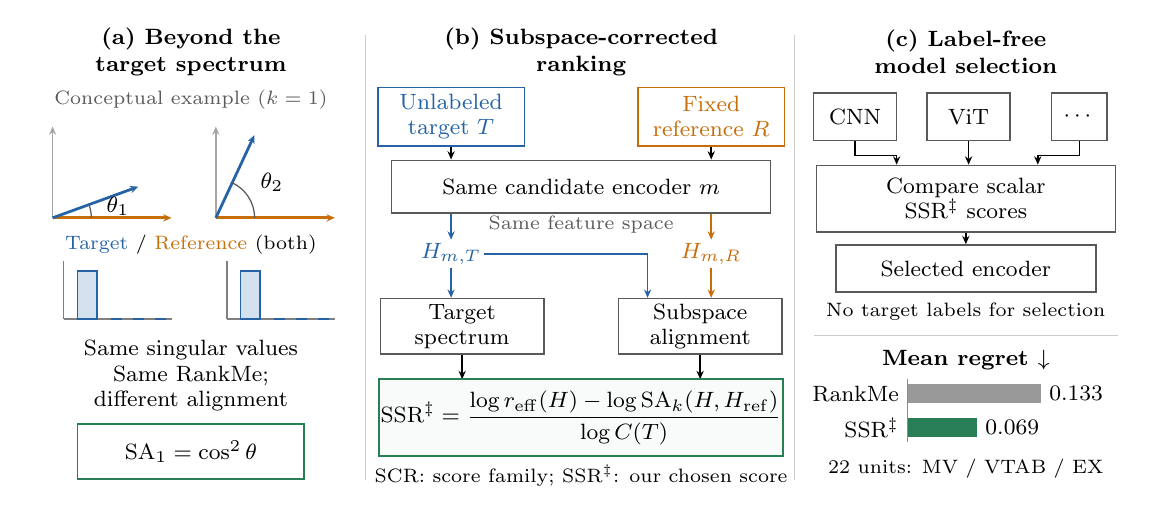
\begin{tikzpicture}[x=1pt,y=.87pt,
  font=\fontsize{8}{9}\selectfont,
  every node/.style={inner sep=1pt,align=center},
  flow/.style={-{Stealth[length=3pt,width=2.6pt]},line width=.55pt},
  box/.style={draw=black!65,line width=.55pt,fill=white},
  head/.style={font=\fontsize{8.5}{10}\selectfont\bfseries}]
\path[use as bounding box] (0,0) rectangle (397.485,190);
\draw[black!20,line width=.45pt] (122,2)--(122,187) (277,2)--(277,187);
\node[head] at (59,180) {(a) Beyond the\\target spectrum};
\node[head] at (200,180) {(b) Subspace-corrected\\ranking};
\node[head] at (339,180) {(c) Label-free\\model selection};

% (a) Identical rank-one spectra, distinct reference-relative geometry.
\node[font=\fontsize{7.5}{9}\selectfont,text=black!65] at (59,160) {Conceptual example ($k=1$)};
\foreach \x/\ang/\idx in {9/20/1,68/65/2}{
  \begin{scope}[shift={(\x,111)},x=1pt,y=1pt]
    \draw[flow,black!35] (0,0)--(0,33);
    \draw[flow,reference,line width=1pt] (0,0)--(43,0);
    \draw[flow,target,line width=1pt] (0,0)--++(\ang:33);
    \draw[black!65,line width=.45pt] (14,0) arc[start angle=0,end angle=\ang,radius=14];
    \node at ({\ang/2}:24) {$\theta_{\idx}$};
  \end{scope}
  \draw[black!50,line width=.45pt] (\x+4,69)--(\x+4,93) (\x+4,69)--(\x+43,69);
  \filldraw[draw=target,fill=target!20,line width=.5pt] (\x+9,69) rectangle (\x+16,89);
  \foreach \dx in {23,31,39} {\draw[target,line width=.8pt] (\x+\dx-2,69)--(\x+\dx+2,69);}
}
\node[font=\fontsize{7.5}{9}\selectfont] at (59,100)
  {\textcolor{target}{Target} / \textcolor{reference}{Reference} (both)};
\node at (59,56) {Same singular values};
\node at (59,40) {Same RankMe;\\different alignment};
\node[draw=score,line width=.7pt,minimum width=82,minimum height=20] at (59,14)
  {$\mathrm{SA}_1=\cos^2\theta$};

% (b) Separate inputs to the same encoder; alignment needs BOTH outputs.
\node[box,draw=target,text=target,minimum width=53,minimum height=21] (T) at (153,153) {Unlabeled\\target $T$};
\node[box,draw=reference,text=reference,minimum width=53,minimum height=21] (R) at (247,153) {Fixed\\reference $R$};
\node[box,minimum width=137,minimum height=19] (enc) at (200,124) {Same candidate encoder $m$};
\draw[flow] (T.south)--(T.south|-enc.north);
\draw[flow] (R.south)--(R.south|-enc.north);
\node[text=target] (HT) at (153,96) {$H_{m,T}$};
\node[text=reference] (HR) at (247,96) {$H_{m,R}$};
\draw[flow,target] (HT.north|-enc.south)--(HT.north);
\draw[flow,reference] (HR.north|-enc.south)--(HR.north);
\node[font=\fontsize{7.5}{9}\selectfont,text=black!65] at (200,108) {Same feature space};
\node[box,minimum width=59,minimum height=20] (spec) at (157,66) {Target\\spectrum};
\node[box,minimum width=59,minimum height=20] (align) at (243,66) {Subspace\\alignment};
\draw[flow,target] (HT.south)--(HT.south|-spec.north);
\draw[flow,reference] (HR.south)--(HR.south|-align.north);
\draw[flow,target] (HT.east)--(224,96)--(224,96|-align.north);
\draw[flow] (spec.south)--(157,44);
\draw[flow] (align.south)--(243,44);
\draw[draw=score,line width=.75pt,fill=score!3] (127,12) rectangle (273,44);
\node at (200,28) {$\displaystyle\mathrm{SSR}^{\ddagger}=\frac{\log r_{\mathrm{eff}}(H)-\log\mathrm{SA}_k(H,H_{\mathrm{ref}})}{\log C(T)}$};
\node[font=\fontsize{7.5}{9}\selectfont] at (200,4) {SCR: score family; SSR$^{\ddagger}$: our chosen score};

% (c) Scalar comparison only; bar lengths use the displayed audited means.
\node[box,minimum width=30,minimum height=17] (cnn) at (299,153) {CNN};
\node[box,minimum width=30,minimum height=17] (vit) at (340,153) {ViT};
\node[box,minimum width=20,minimum height=17] (etc) at (380,153) {$\cdots$};
\node[box,minimum width=108,minimum height=24] (rank) at (339,119) {Compare scalar\\SSR$^{\ddagger}$ scores};
\draw[flow] (cnn.south)--(299,137)--(314,137)--(314,137|-rank.north);
\draw[flow] (vit.south)--(vit.south|-rank.north);
\draw[flow] (etc.south)--(380,137)--(365,137)--(365,137|-rank.north);
\node[box,minimum width=94,minimum height=17] (selected) at (339,90) {Selected encoder};
\draw[flow] (rank.south)--(selected.north);
\node[font=\fontsize{7.5}{9}\selectfont] at (339,72) {No target labels for selection};
\draw[black!20,line width=.45pt] (284,62)--(394,62);
\node[font=\fontsize{8}{9}\selectfont\bfseries] at (339,52) {Mean regret $\downarrow$};
\node[anchor=east] at (316,38) {RankMe};
\node[anchor=east] at (316,24) {SSR$^{\ddagger}$};
\draw[black!45,line width=.4pt] (318,18)--(318,44);
\fill[black!40] (318,34) rectangle (366,42);
\fill[score] (318,20) rectangle ({318+48*.069/.133},28);
\node[anchor=west] at (368,38) {0.133};
\node[anchor=west] at ({320+48*.069/.133},24) {0.069};
\node[font=\fontsize{7.5}{9}\selectfont] at (339,7) {22 units: MV / VTAB / EX};
\end{tikzpicture}
\end{document}
